\section{Methods}

Our method incorporates two types of signal from the data -- change in number of fragments sequenced from a particular region, and change of the allele distributions at SNP loci inside the region. In what follows, we first describe each signal processing separately and later show how we combine them into a joint prediction.

\subsection{CNV calling based on sequencing coverage}
Sequencing of cell-free DNA carries sequencing biases other then just GC content when compared to standard WGS. \cite{srinivasan2013}


\subsection{Hidden Markov Model for CNVs Inference}\label{ss:hmm}
To combine the signals form individual SNP positions, we use a hidden Markov model. For each inheritance pattern we use a model like in Figure \ref{fig:model}, to compute likelihood of the observed samples under assumption of such inheritance pattern. To the possible inheritance patterns correspond the states of the HMM (for each SNP position) with emission probabilities proportional to the likelihood. See Figure \ref{fig:hmm}. As the likelihood which we get from the graphical model is already probability, we can interpret it right away as the emission probability. In practice we add some small positive constant $\varepsilon$ to these probabilities (and then normalize) to account for noise in the data.

\begin{figure}[h!]
%\center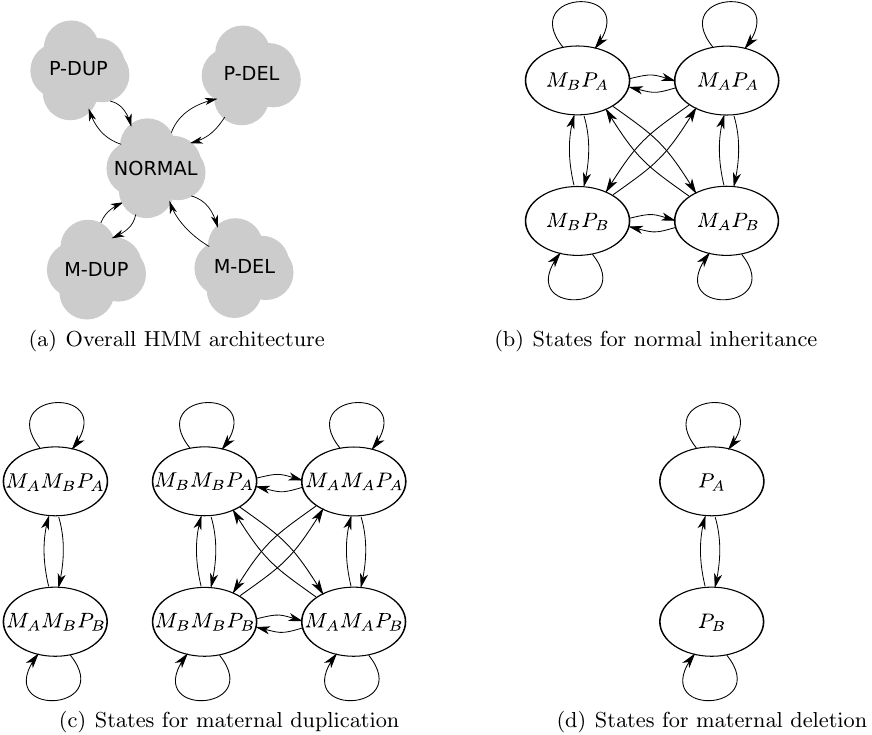
\includegraphics[width = 0.95\textwidth]{hmm}
\caption{Hidden Markov model used for CNV inference. We do not allow two CNVs to be adjacent, thus the switching always has to go through ``1M 1P'' (normal) state. The thicker arrows signalize higher transition probability to stay in the particular inheritance pattern.}\label{fig:hmm}
\end{figure}

The HMM as depicted in Figure \ref{fig:hmm} is in a more general form, when we allow for different transition probabilities, depending on the given SNP site. This is useful if we want to model for non-uniform distance between individual SNPs. However in this project we assume uniform distribution and thus the transition probabilities are independent of actual position.

The initial transition probabilities are set to reflect that we expect one CNV event to span multiple SNP positions. We set the initial probability of changing the current inheritance pattern to 0.001 and the probability of staying to the rest. That means a priori we expect CNVs to span 1000 SNPs and be 1000 SNPs one from each other.

We then train the transition probabilities separately by Baum-Welsh algorithm and by Viterbi training \cite{durbin1998}. Obtained results can be found in Section Results, where we infer the CNVs by both Viterbi decoding and maximum posterior decoding.